% This text is Free and open Open Source.
% It's a part of presentation made by myself.
% It may be used only for academic purpose
% May, 2012
% Author: Seshagiri Prabhu
% Amrita Vishwa Vidyapeethm 
% seshagiriprabhu@gmail.com
% www.seshagiriprabhu.wordpress.com

\documentclass[12pt]{beamer}
\usetheme{Oxygen}
\usepackage{thumbpdf}
\usepackage{wasysym}
\usepackage{ucs}
\usepackage[utf8]{inputenc}\usepackage{pgf,pgfarrows,pgfnodes,pgfautomata,pgfheaps,pgfshade}
\usepackage{verbatim}
\usepackage{listings}
\usepackage{courier}
\usepackage{caption}
\usepackage{verbatim} 
\usepackage{upquote}
\usepackage{graphics}
\usepackage{latexsym}
\usepackage{fixltx2e}
\usepackage{graphicx}
\usepackage{hyperref}
\usepackage{amssymb}
\usepackage{ragged2e}
\usepackage{amsmath}
\usepackage{mathtools}
\usepackage{framed,lipsum}
\usepackage{pgf}
\usepackage{fmtcount}% http://ctan.org/pkg/fmtcount
\usepackage{algorithm, algpseudocode}
\usepackage{caption}
\captionsetup[algorithm]{font=scriptsize}
\usepackage{etoolbox}
\makeatother
\newcommand\Colorhref[3][cyan]{\href{#2}{\small\color{#1}#3}}
\newcommand\Fontvi{\fontsize{5}{6}\selectfont}
%\renewcommand\tinyv{\@setfontsize\tinyv{4pt}{6}}
%\renewcommand\tiny{\@setfontsize\tiny{4pt}{6}}
\usepackage{color}

\usepackage{xcolor}

\def\SPSB#1#2{\rlap{\textsuperscript{\textcolor{red}{#1}}}\SB{#2}}
\def\SP#1{\textsuperscript{\textcolor{red}{#1}}}
\def\SB#1{\textsubscript{\textcolor{blue}{#1}}}
\setbeamertemplate{itemize items}[default]
\setbeamertemplate{enumerate items}[default]
\usepackage{listings}
\usepackage{color}

\definecolor{mygreen}{rgb}{0,0.6,0}
\definecolor{mygray}{rgb}{0.5,0.5,0.5}
\definecolor{mymauve}{rgb}{0.58,0,0.82}
\lstset{
 breaklines=true, commentstyle=\color{mygreen}, stepnumber=1, tabsize=2, stringstyle=\color{mymauve}, numberstyle=\tiny\color{mygray}, rulecolor=\color{black}, morekeywords={make,mkdir,gcc, all, clean, F, OO}, basicstyle=\tiny\ttfamily,keywordstyle=\color{blue}, emph={CC, CFLAG, EXECS, PROG, OBJS, OBJECTS, PHONY}, emphstyle=\color{red}, emph={[2]\#using,\#define,\#ifdef,\#endif}, emphstyle={[2]\color{blue}}, stringstyle=\color{red}
}
\newenvironment{variableblock}[3]{%
  \setbeamercolor{block body}{#2}
  \setbeamercolor{block title}{#3}
  \begin{block}{#1}}{\end{block}}
\pdfinfo
{
  /Title       (SN 707 Software Protection)
  /Creator     (Seshagiri Prabhu N)
  /Author      (TeX)
}
\title{CS620 Advanced Computer Networks}
\subtitle{Lab 1}
\author{Course Mentor: Snehal Shetty \\ TA: Seshagiri Prabhu}
\institute[Amrita Vishwa Vidyapeetham] % (optional)
{
  \begin{center}
    \tiny
    Amrita Center for Cyber Security\\
	Amritapuri
  \end{center}  
}

\begin{document}
\frame{\titlepage}
\begin{frame}
	\begin{variableblock}{}{bg=orange,fg=black}{bg=green,fg=red}
		\begin{center}
			\vskip5mm
  			{\large Socket Programming in C}
  			\vskip5mm
  			\vskip5mm  			
		\end{center}
	\end{variableblock}
\end{frame}

\begin{frame}
	{\large Contact info}
	\begin{center}
		{\large Snehal Shetty} \\
		{\small \textcolor{blue}{Office}} \\
		{\small \textcolor{black}{103}} \\
		\vskip1mm
		{\small \textcolor{blue}{email}} \\
		{\small \href{mailto:snehal@am.amrita.edu}{snehal@am.amrita.edu}}\\
		\vskip5mm
		{\large Seshagiri Prabhu} \\
		{\small \textcolor{blue}{Office}} \\		
		{\small \textcolor{black}{110}} \\		
		\vskip1mm
		{\small \textcolor{blue}{email}} \\
		{\small \href{mailto:seshagiriprabhu@am.amrita.edu}{seshagiriprabhu@am.amrita.edu}}\\
	\end{center}
\end{frame}

\begin{frame}
  \frametitle{Outline}
  \tableofcontents[section=1,hidesubsections]
\end{frame}

\newcommand{\icon}[1]{\pgfimage[height=1em]{#1}}

%%%%%%%%%%%%%%%%%%%%%%%%%%%%%%%%%%%%%%%%%
%%%%%%%%%% Content starts here %%%%%%%%%%
%%%%%%%%%%%%%%%%%%%%%%%%%%%%%%%%%%%%%%%%%

\section{Socket}
\begin{frame}
	\frametitle{Sockets}
	{\small Sockets are a protocol independent method of creating a connection between processes. Sockets can be either}
	\begin{itemize}
		\item \textcolor{red}{connection based} or \textcolor{red}{connectionless}: Is a connection established before communication or does each packet describe the destination?
		\item \textcolor{red}{packet based} or \textcolor{red}{streams based}: Are there message boundaries or is it one stream?
		\item \textcolor{red}{reliable} or \textcolor{red}{unreliable}. Can messages be lost, duplicated, reordered, or corrupted?
	\end{itemize}
\end{frame}

%\begin{frame}
%	\frametitle{Socket Characteristics}
%	{\small Socket are characterized by their domain, type and transport protocol. Common domains are:}
%	\begin{itemize}
%		\item \color{blue}{AF_UNIX}:address format is UNIX pathname	
%	\end{itemize}
%\end{frame}
\begin{frame}
	\frametitle{Socket Characteristics}
	{\small Socket are characterized by their domain, type and transport protocol. Common domains are:}
	\begin{itemize}
		\item \textcolor{blue}{\texttt{AF\_UNIX}}: address format is UNIX pathname
		\item \textcolor{blue}{\texttt{AF\_INET}}: address format is host and port number
	\end{itemize}
	\vskip4mm
	{\small Common types are:}
	\begin{itemize}
		\item \textcolor{blue}{Virtual Circuits}: received in order transmitted and reliably
		\item \textcolor{blue}{datagram}: arbitrary order, unreliable
	\end{itemize}
\end{frame}

\begin{frame}
	\frametitle{Socket Characteristics (cont'd)}
	{\small Each socket type has one or more protocols. Ex:}
	\begin{itemize}
		\item TCP/IP (virtual circuits)
		\item UDP (datagram)
	\end{itemize}
	\vskip4mm
	{\small Use of sockets:}
	\begin{itemize}
		\item Connection–based sockets communicate client-server: the server waits for a connection from the client.
		\item Connectionless sockets are peer-to-peer: each process is symmetric.
	\end{itemize}
\end{frame}

\begin{frame}
	\frametitle{Socket APIs}
	\begin{itemize}
		\item \textcolor{blue}{\texttt{socket}}: creates a socket of a given domain, type, protocol
(buy a phone)
		\item \textcolor{blue}{\texttt{listen}}: assigns a name to the socket (get a telephone number)
		\item \textcolor{blue}{\texttt{accept}}: specifies the number of pending connections that can be queued for a server socket. (call waiting allowance)
		\item \textcolor{blue}{\texttt{connect}}: client requests a connection request to a server
(call)	
		\item \textcolor{blue}{\texttt{send, sendto}}: write to connection (speak)
		\item \textcolor{blue}{\texttt{recv, recvfrom}}: read from connection (listen)		
		\item \textcolor{blue}{\texttt{shutdown}}: end the call	
	\end{itemize}
\end{frame}

\section{TCP}
\begin{frame}
	\frametitle{Connection based communication}
	{\small Server performs these actions:}
	\begin{itemize}
		\item \textcolor{blue}{\texttt{socket}}: create the socket
		\item \textcolor{blue}{\texttt{bind}}: give the address of the socket on the server
		\item \textcolor{blue}{\texttt{listen}}: specifies the maximum number of connection requests that can be pending for this process
		\item \textcolor{blue}{\texttt{accept}}: establish the connection with a specific client
		\item \textcolor{blue}{\texttt{send, recv}}: stream-based equivalents of read and write
		\item \textcolor{blue}{\texttt{shutdown}}: end reading or writing
		\item \textcolor{blue}{\texttt{listen}}: release kernel data structures
	\end{itemize}
\end{frame}

\begin{frame}
	\frametitle{TCP-based sockets}
	\begin{center}
		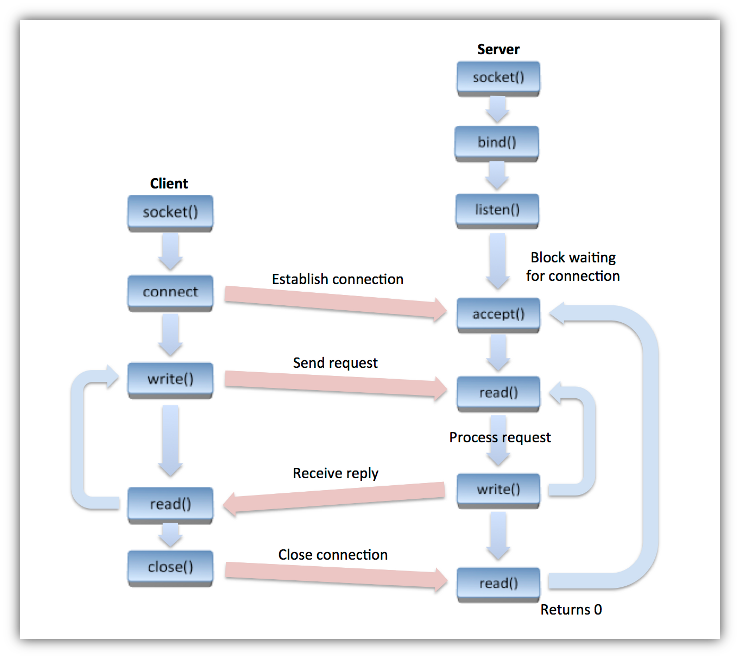
\includegraphics[scale=.65]{images/Socket-Workflow.png} 
	\end{center}
\end{frame}

\begin{frame}[fragile]
	\frametitle{socket API}
	{\tiny
	\begin{lstlisting}[language=C, breaklines=true, commentstyle=\color{mygreen},frame=lrtb,  rulecolor=\color{black}, numbers=left,  numbersep=5pt, numberstyle=\tiny\color{mygray}]
	#include <sys/types.h>
	#include <sys/socket.h>
	int socket(int domain, int type, int protocol);
	\end{lstlisting}}
	{\footnotesize
	Returns a file descriptor (called socket ID) if successful, -1 otherwise. Note that the socket returns a socket descriptor which is the same as a file descriptor. \\
	The \textcolor{blue}{domain} is \textcolor{blue}{\texttt{AF\_INET}}. \\
	The \textcolor{blue}{type} argument can be: \\
	\begin{itemize}
		\item \textcolor{blue}{\texttt{SOCK\_STREAM}}: Establishes a virtual circuit for stream
		\item \textcolor{blue}{\texttt{SOCK\_DGRAM}}: Establishes a datagram for communication 
		\item \textcolor{blue}{\texttt{SOCK\_SEQPACKET}}:  Establishes a reliable, connection based,
two way communication with maximum message size. (This is not available on most machines.)
	\end{itemize}
	\textcolor{blue}{protocol} is usually \textcolor{red}{zero}, so that \textcolor{blue}{type} defines the connection 	within domain.
	}
\end{frame}

\begin{frame}[fragile]
	\frametitle{bind}
	{\tiny
	\begin{lstlisting}[language=C, breaklines=true, commentstyle=\color{mygreen},frame=lrtb,  rulecolor=\color{black}, numbers=left,  numbersep=5pt, numberstyle=\tiny\color{mygray}]
	#include <sys/types.h>
	#include <sys/socket.h>
	int bind(int sockfd, const struct sockaddr *addr,
                socklen_t addrlen);
	\end{lstlisting}}
	{\footnotesize
	where 
	\begin{itemize}
		\item \texttt{\textcolor{blue}{sockfd}}: is the socket id.
		\item \texttt{\textcolor{blue}{addr}}: is a pointer to the address family dependant address structure,
		\item \texttt{\textcolor{blue}{addrlen}}: is the len of \texttt{\textcolor{blue}{$\ast$addr}}
	\end{itemize}
	Associates a socket id with an address to which other processes can connect. In internet protocol the address is [ipNumber, portNumber]
	}
\end{frame}

\begin{frame}[fragile]
	\frametitle{sockaddr}
	{\footnotesize For the internet family:}
	{\tiny
	\begin{lstlisting}[language=C, breaklines=true, commentstyle=\color{mygreen},frame=lrtb,  rulecolor=\color{black}, numbers=left,  numbersep=5pt, numberstyle=\tiny\color{mygray}]
	#include <sys/types.h> 
	#include <sys/socket.h>
	int listen(int sockfd, int backlog);
	\end{lstlisting}}
	{\footnotesize
	Where \texttt{\textcolor{blue}{backlog}} it the number of pending connection requests allowed (typically limited by Unix kernels to 5). \\ Returns the 0 on success, or -1 if failure.
	}
\end{frame}

\begin{frame}[fragile]
	\frametitle{accept}
	{\tiny
	\begin{lstlisting}[language=C, breaklines=true, commentstyle=\color{mygreen},frame=lrtb,  rulecolor=\color{black}, numbers=left,  numbersep=5pt, numberstyle=\tiny\color{mygray}]
	#include <sys/types.h>
	#include <sys/socket.h>
	int accept(int sockfd, struct sockaddr *addr, 
	           socklen_t *addrlen);
	\end{lstlisting}}
	{\footnotesize
	Returns the socketId and address of client connecting to socket. if \texttt{\textcolor{blue}{addrlen}} or \texttt{\textcolor{blue}{addr}} equal zero, no address structure is returned. \texttt{\textcolor{blue}{addrlen}} is the maximum size of address structure that can be called, returns the actual value. \\Waits for an incoming request, and when received creates a socket for it.
	}
\end{frame}

\begin{frame}
	\frametitle{accept styles}
	{\footnotesize
	There are basically three styles of using accept:
	\begin{itemize}
		\item \textcolor{blue}{Iterating server:} Only one socket is opened at a time. When the processing on that connection is completed, the socket is closed, and next connection can be accepted.
		\item \textcolor{blue}{Forking server}: After an accept, a child process is forked off to handle the connection. Variation: the child processes are preforked and are passed the socketId.
		\item \textcolor{blue}{Concurrent single server}: use select to simultaneously wait on all open socketIds, and waking up the process only when new data arrives.
	\end{itemize}
	}
\end{frame}

\begin{frame}
	\frametitle{Pro and con of accept styles}
	{\footnotesize

	\begin{itemize}
		\item \textcolor{blue}{Iterating server} is basically a low performance technique since
only one connection is open at a time.
		\item \textcolor{blue}{Forking servers} enable using multiple processors. But they
make sharing state difficult, unless performed with threads.
Threads, however present a very fragile programming
environment.
		\item \textcolor{blue}{Concurrent single server}: reduces context switches relative to
forking processes and complexity relative to threads. But does
not benefit from multiprocessors.
	\end{itemize}
	}
\end{frame}

\begin{frame}[fragile]
	\frametitle{send}
	{\tiny
	\begin{lstlisting}[language=C, breaklines=true, commentstyle=\color{mygreen},frame=lrtb,  rulecolor=\color{black}, numbers=left,  numbersep=5pt, numberstyle=\tiny\color{mygray}]
	#include <sys/types.h>
	#include <sys/socket.h>
	ssize_t send(int sockfd, const void *buf, 
	             size_t len, int flag);
	\end{lstlisting}}
	{\footnotesize
	Send a message. Returns the number of bytes sent or -1 if failure. (Must be a bound socket). \\ flag is either
	\begin{itemize}
	\item 0: default
	\item \texttt{\textcolor{blue}{MSG\_OOB}}: Out-of-band high priority communication	
	\end{itemize}
	}
\end{frame}

\begin{frame}[fragile]
	\frametitle{recv}
	{\tiny
	\begin{lstlisting}[language=C, breaklines=true, commentstyle=\color{mygreen},frame=lrtb,  rulecolor=\color{black}, numbers=left,  numbersep=5pt, numberstyle=\tiny\color{mygray}]
	#include <sys/types.h>
	#include <sys/socket.h>
	ssize_t recv(int sockfd, void *buf, 
	             size_t len, int flags);
	\end{lstlisting}}
	{\footnotesize
	Receive up to \texttt{\textcolor{blue}{len}} bytes in \texttt{\textcolor{blue}{bufferPtr}}. Returns the number of bytes received or -1 on failure. \\ flags can be either

	\begin{itemize}
	\item 0: default
	\item \texttt{\textcolor{blue}{MSG\_OOB}}:  out-of-bound message
	\item \texttt{\textcolor{blue}{MSG PEEK}}: look at message without removing
	\end{itemize}
	}
\end{frame}

\begin{frame}[fragile]
	\frametitle{shutdown}
	{\tiny
	\begin{lstlisting}[language=C, breaklines=true, commentstyle=\color{mygreen},frame=lrtb,  rulecolor=\color{black}, numbers=left,  numbersep=5pt, numberstyle=\tiny\color{mygray}]
	#include <sys/types.h>
	#include <sys/socket.h>
	int shutdown(int sockfd, int how);
	\end{lstlisting}}
	{\footnotesize
	Disables sending (how=1 or how=2) or receiving (how=0 or how=2). Returns -1 on failure. \\ acts as a partial close.
	}
\end{frame}

\begin{frame}[fragile]
	\frametitle{connect}
	{\tiny
	\begin{lstlisting}[language=C, breaklines=true, commentstyle=\color{mygreen},frame=lrtb,  rulecolor=\color{black}, numbers=left,  numbersep=5pt, numberstyle=\tiny\color{mygray}]
	#include <sys/types.h>
	#include <sys/socket.h>
	int connect(int sockfd, const struct sockaddr *addr,
	            socklen_t addrlen);
	\end{lstlisting}}
	{\footnotesize
	Specifies the destination to form a connection with (addr), and returns a 0 if successful, -1 otherwise.
	}
\end{frame}	

\begin{frame}
	\frametitle{Denoting Connections}
	{\footnotesize Note that a connection is denoted by a 5-tuple:
	\begin{itemize}
		\item source IP
		\item source port
		\item protocol
		\item destination IP
		\item destination port
	\end{itemize}sockaddr in serverAddr ;
	So that multiple connections can share the same IP and port.
	}
\end{frame}

\begin{frame}
	\frametitle{Port usage}
	{\footnotesize Note that the initiator of communications needs a fixed port to
target communications. This means that some ports must be reserved for these “well known” ports. \\Port usage:
	\begin{itemize}
		\item 0-1023: These ports can only be binded to by root
		\item 1024-5000: well known ports
		\item 5001-64K-1: ephemeral ports
	\end{itemize}
	}
\end{frame}

\begin{frame}[fragile]
	\frametitle{Example: TCP/IP Server Code}	
	{\tiny
	\begin{lstlisting}[language=C, breaklines=true, commentstyle=\color{mygreen},frame=lrtb,  rulecolor=\color{black}, numbers=left,  numbersep=5pt, numberstyle=\tiny\color{mygray}]
sockaddr in serverAddr ;
sockaddr &serverAddrCast = (sockaddr &)serverAddr;

//get a tcp/ip socket
int listenFd = socket (AF_INET , SOCK_STREAM , 0);

bzero (&serverAddr , sizeof (serverAddr));
serverAddr.sinfamily = AF_INET;

//any internet interface on this server 
serverAddr.sinaddr.saddr = htonl (INADDR_ANY);
serverAddr.sin_port = htons(13);

bind(listenFd, &serverAddrCast, sizeof(serverAddr));

listen(listenFd, 5);

for ( ; ; ) {
    int connectFd =
        accept (listenFd, ( sockaddr * ) NULL, NULL);
        // .... read and write operations on connectFd
    shutdown(connectFd, 2);
    close(connectFd);
}
	\end{lstlisting}}
	{\footnotesize
	Note that the above is an \textcolor{red}{iterative server}, which means that it serves one connection at a time.
	}
\end{frame}	

\begin{frame}
	\frametitle{Concurrent Server}
	{\footnotesize To build a concurrent server::
	\begin{itemize}
		\item a fork is performed after the accept.
		\item The child process closes listenFd, and communicates using connectFd. 
		\item The parent process closses connectFd, and then loops back to the accept to wait for another connection request
	\end{itemize}
	}
\end{frame}

\begin{frame}[fragile]
	\frametitle{Example: TCP/IP Server Code}	
	{\tiny
	\begin{lstlisting}[language=C, breaklines=true, commentstyle=\color{mygreen},frame=lrtb,  rulecolor=\color{black}, numbers=left,  numbersep=5pt, numberstyle=\tiny\color{mygray}]
sockaddr in serverAddr ;
sockaddr &serverAddrCast = (sockaddr &)serverAddr;

// get a tcp/ip socket
int sockFd = socket (AF_INET , SOCK_STREAM , 0);

bzero (&serverAddr , sizeof (serverAddr));
serverAddr.sinfamily = AF_INET;

// host IP # in dotted decimal format
inet_pton(AF_INET, serverName, serverAddr.sin_addr);
serverAddr.sin_port = htons(13);

connect(sockFd, serverAddrCast, sizeof(serverAddr));
      // ... read and write operations on sockFd ..
     
shutdown(socktFd, 2);
close(sockFd);
}
	\end{lstlisting}}
	{\footnotesize
	Note that the above is an \textcolor{red}{concurrent server}, which means that it can serves more than one connection at a time.
	}
\end{frame}	

\begin{frame}[fragile]
	\frametitle{Problem Description}
	\framesubtitle{Compile and run the program}
	\tiny
	\begin{block}{Compile the program}
		\begin{lstlisting}[language=bash]
seshagiri@ACCS:~$ make
mkdir -p OBJECTS
gcc -c -Wall circle.c -o OBJECTS/circle.o
gcc OBJECTS/circle.o -o circle
    	\end{lstlisting}
    \end{block}
    
	\begin{block}{Execute the binary file - $circle$}
		\begin{lstlisting}[language=bash]
seshagiri@ACCS:~$ ./circle
0.250
		\end{lstlisting}
	\end{block}
\end{frame}

\begin{frame}
	\frametitle{Problem Description}
	\framesubtitle{What can we understand after executing the binary file?}
	\begin{center}
		\small What can we understand after executing the binary file?
		\small{$<burp>$} \huge {NOTHING!} \small {$</burp>$}
	\end{center}
\end{frame}

\begin{frame}
	\frametitle{Problem Description}
	\framesubtitle{What should we do next?}
	\begin{center}
		\small {What should we do next?} \\
		\large Inspect the source code
	\end{center}
\end{frame}

\begin{frame}[fragile]
	\frametitle{Problem Description}
	\framesubtitle{Intended the code properly for better understanding}
	\begin{lstlisting}[language=C, breaklines=true, commentstyle=\color{mygreen}, rulecolor=\color{black}, numbers=left,  numbersep=2pt, numberstyle=\tiny\color{mygray}] ]
#include <stdio.h>
#define _ -F<00||--F-OO--;

int F=00,OO=00;

main() {
        F_OO();
        printf("%1.3f\n", 4.*-F/OO/OO);
}

F_OO() {
            _-_-_-_
       _-_-_-_-_-_-_-_-_
    _-_-_-_-_-_-_-_-_-_-_-_
  _-_-_-_-_-_-_-_-_-_-_-_-_-_
 _-_-_-_-_-_-_-_-_-_-_-_-_-_-_
 _-_-_-_-_-_-_-_-_-_-_-_-_-_-_
_-_-_-_-_-_-_-_-_-_-_-_-_-_-_-_
_-_-_-_-_-_-_-_-_-_-_-_-_-_-_-_
_-_-_-_-_-_-_-_-_-_-_-_-_-_-_-_
_-_-_-_-_-_-_-_-_-_-_-_-_-_-_-_
 _-_-_-_-_-_-_-_-_-_-_-_-_-_-_
 _-_-_-_-_-_-_-_-_-_-_-_-_-_-_
  _-_-_-_-_-_-_-_-_-_-_-_-_-_
    _-_-_-_-_-_-_-_-_-_-_-_
        _-_-_-_-_-_-_-_
            _-_-_-_
}
	\end{lstlisting}

\end{frame}

\section{Problem Dissection}
\begin{frame}[fragile]
	\frametitle {Problem Dissection}
	\framesubtitle {Macro... Macro..}
	\begin{block}{Unnoticed macro $\_$ }
		\begin{lstlisting}[language=C]
			#define _ -F<00||--F-OO--;
		\end{lstlisting}	
	\end{block}
	\begin{block}{What macro does?}
		\begin{itemize}
			\item Replaces '\texttt{\_}' with {\tiny '\texttt{-F<00||-{}-F-OO-{}-;}'}
			\item for eg: {\tiny '\texttt{\_-\_-\_}'} becomes {\tiny '\texttt{-F<00||-{}-F-OO-{}-;- -F<00||-{}-F-OO-{}-;- -F<00||-{}-F-OO-{}-;}'}
			\item One of the important property of \texttt{||} operator is that if the first condition is \textcolor{red}{true}, it will \textcolor{red}{NOT} check for the second condition unlike \texttt{\&\&} operator.
		\end{itemize}
	\end{block}
\end{frame}

\begin{frame}[fragile]
	\frametitle{Problem Dissection}
	\framesubtitle{Values of variables inside \texttt{F\_OO()}}
	\begin{block}{Values of \texttt{F} and \texttt{OO}}
		\begin{itemize}
			\item \texttt{F} and \texttt{OO} are initially set as $zero$. 
			\item In the first line of \texttt{F\_OO} function, \texttt{-F<00} becomes \textcolor{red}{false} hence checks for the second condition.
			\item \texttt{-{}-F} becomes -1 and \texttt{OO-{}-} remains as 0.
			\item After the execution of the first line, value of F becomes -1 and OO becomes -1.
		\end{itemize}				
	\end{block}
\end{frame}

\begin{frame}[fragile]
	\frametitle{Problem Dissection}
	\framesubtitle{Values of \texttt{F} and \texttt{OO} inside \texttt{F\_OO()}}
	\begin{itemize}
	\item  {\tiny \textbf{Line 1:} texttt{-0<0 (\textcolor{red}{false}) || (-1)-(0--) (\textcolor{green}{executed}); -1<0 (\textcolor{green}{true}) || (-2)-(-1)(\textcolor{red}{not executed}); -1 < 0 (\textcolor{green}{true}) || (-3)-(-2)(\textcolor{red}{not executed})}}. {\tiny \texttt{F = -1, OO = -1}}
	\item {\tiny \textbf{Line 2:} \texttt{1<0 (\textcolor{red}{false}) || (-2)-(1--) (\textcolor{green}{executed}); -2<0 (\textcolor{green}{true}) || (-3)-(-2)(\textcolor{red}{not executed}); -3 < 0 (\textcolor{green}{true}) || (-4)-(-3)(\textcolor{red}{not executed}) -4<0 (\textcolor{green}{true}) || (-5)-(-4)(\textcolor{red}{not executed}); -5 < 0 (\textcolor{green}{true}) || (-6)-(-5)(\textcolor{red}{not executed})}}. {\tiny \texttt{F = -2, OO = -2}}
	\\.
	\\.
	\\.
	\item {\tiny \textbf{Line 16:} \texttt{F = -16, OO = -16} }
	\end{itemize}
\end{frame}

\begin{frame}[fragile]
	\frametitle{Problem Dissection}
	\framesubtitle{Lets go back to \texttt{main()} where \texttt{F\_OO()} was called}
	\begin{block}{Inside \texttt{main()}}
		\begin{lstlisting}[language=C]
			printf("%1.3f\n",4.*-F/OO/OO);
		\end{lstlisting}
		This line calculates the value 0.250 
	\end{block}
\end{frame}

\begin{frame}
	\frametitle{Problem Dissection}
	\framesubtitle{What was the learning from this program?}
	\begin{center}
		\small {What was the learning by inspecting the code} \\
		\huge {NIL}
	\end{center}
\end{frame}

\begin{frame}
	\frametitle{Problem Dissection}
	\framesubtitle{What should be done next?}
	\begin{center}
		\small {What should be done next?} \\
		\small {Lets} \\
	\end{center}
\end{frame}

\begin{frame}
	\frametitle{Problem Dissection}
	\framesubtitle{What should be done next?}
	\begin{center}
		\small {Bingo! Wiki rocks} \\
		{\tiny \url{http://en.wikipedia.org/wiki/International_Obfuscated_C_Code_Contest\#Examples}}
		{\tiny The same example is mentioned in the above mentioned link and it says that the program works by calculating its own area and diameter, and then doing a division to approximate pi!!} \\
		{\small They call it as an Obfuscated C code}
	\end{center}
\end{frame}

\begin{frame}
	\frametitle{Problem Dissection}
	\framesubtitle{How does it calculates the value of $\Pi$?}
	\begin{block}{Lets do reverse engineering!}
		Using the hint in Wiki, we found that program works by calculating its own area and diameter. So we need to make the $\Pi$, Area, radius/diameter looks like \texttt{4.*-F/OO/OO}. \\ So lets do reverse Engineering!
	\end{block}
\end{frame}

\begin{frame}
	\frametitle{Problem Dissection}
	\framesubtitle{Calculating the value of $\Pi$ }
	\begin{block}{Calculating the value of $\Pi$ from Area and radius/diameter}
		Area = $\Pi$ * $radius^{2}$ \\
		$\Pi$ = Area / $radius^{2}$ \\
		As we need 4 in the numerator we may have to substitute radius with diameter.\\
		$\Pi$ = Area / $(diameter/2)^{2}$ \\
		$\Pi$ = 4 * Area / (diameter * diameter) \\
		$\Pi$ = 4 * Area / diameter / diameter \\
	\end{block}
\end{frame}	

\section{Inference}
\begin{frame}
	\frametitle{Inference}
	\framesubtitle{What can we conclude from this?}
	\begin{block}{Conclusion}
		Variable \textcolor{red}{F} is the area of the circle used in the program \\
		The Diameter of the circle is the variable \textcolor{red}{OO}
	\end{block}
\end{frame}

\begin{frame}
	\frametitle{Learning}
	\framesubtitle{What's new I have learned from this?}
	\begin{block}{Learning something new}
		Previously, I have tried to de-obfuscating PHP code (in which they used base64 encoding, rot 13 transformation etc) files during Capture The Flag contests. This is the first time I am hearing about C code obfuscation. That was a nice learning experience!
	\end{block}
\end{frame}

\frame{
  	\vspace{2cm}
	\begin{center}
  		{\huge Thank you!}
	\end{center}
  	\vspace{1cm}
  	\begin{flushright}
        Seshagiri Prabhu \\
    	\structure{\footnotesize{seshagiriprabhu@gmail.com} \\ AM.EN.P2CSN12028 \\  \href{https://github.com/seshagiriprabhu/software-protection-lab}{Assignment repo}}
  	\end{flushright}
}

\end{document}